\documentclass[12pt]{report}

% greek hyphenation package
\usepackage{fontspec}
\usepackage{xgreek}
\usepackage{amsmath}
\usepackage{amsfonts}
\usepackage{amssymb}
\usepackage{bm}

\newcommand{\norm}[1]{\left\lVert #1 \right\rVert_2}
\newcommand{\abs}[1]{\left\vert #1 \right\vert}

\usepackage{fancyhdr}
\usepackage{sectsty}

\usepackage{array}
\usepackage{multirow}
\usepackage{adjustbox}
\usepackage{hyperref}
\hypersetup{
    colorlinks=true,
    linkcolor=blue,
    filecolor=magenta,
    urlcolor=cyan,
}



\usepackage{float}
\usepackage{framed}
\restylefloat{table}

\usepackage[utf8]{inputenc}
\usepackage{algorithm,algorithmicx,algpseudocode}

\algnewcommand{\LineComment}[1]{\State \# #1}
\renewcommand{\algorithmicrequire}{\textbf{Input:}}
\renewcommand{\algorithmicensure}{\textbf{Output:}}

\usepackage[margin=1in,footskip=0.40in]{geometry}

\usepackage{listings}
\usepackage{xcolor}

\usepackage{graphicx}
\usepackage[justification=centering,labelfont=bf]{caption}
\usepackage{subcaption}
\graphicspath{{images/}}

\usepackage{datetime}
\usepackage{polyglossia}
\setmainlanguage{greek}

\setlength{\parindent}{4em}
\setlength{\parskip}{1em}

\usepackage[normalem]{ulem}
\usepackage[uppercase]{titlesec}

\allsectionsfont{\centering}
\titleformat{\chapter}
{\Huge\bfseries\filcenter}{\uline{\thechapter.\ }}{0em}{\uline}
\titleformat{\section}
{\Large\bfseries\filcenter}{\uline{\thesection.\ }}{0em}{\uline}
\titleformat{\subsection}{\large\filcenter}{\uline{\thesubsection.\ }}{0em}{\uline}
\titleformat{\subsubsection}{\normalsize\filright}{\uline{\thesubsubsection.}}{0em}{\uline}
\setmainfont[Mapping=tex-text]{DejaVu Sans}
\newfontfamily\greekfont[Script=Greek]{DejaVu Sans}

\usepackage{listings}
\usepackage{xcolor}

\definecolor{mygreen}{rgb}{0,0.6,0}
\definecolor{mygray}{rgb}{0.5,0.5,0.5}
\definecolor{mymauve}{rgb}{0.58,0,0.82}

\lstset{literate=
  {á}{{\'a}}1 {é}{{\'e}}1 {í}{{\'i}}1 {ó}{{\'o}}1 {ú}{{\'u}}1
  {Á}{{\'A}}1 {É}{{\'E}}1 {Í}{{\'I}}1 {Ó}{{\'O}}1 {Ú}{{\'U}}1
  {à}{{\`a}}1 {è}{{\`e}}1 {ì}{{\`i}}1 {ò}{{\`o}}1 {ù}{{\`u}}1
  {À}{{\`A}}1 {È}{{\'E}}1 {Ì}{{\`I}}1 {Ò}{{\`O}}1 {Ù}{{\`U}}1
  {ä}{{\"a}}1 {ë}{{\"e}}1 {ï}{{\"i}}1 {ö}{{\"o}}1 {ü}{{\"u}}1
  {Ä}{{\"A}}1 {Ë}{{\"E}}1 {Ï}{{\"I}}1 {Ö}{{\"O}}1 {Ü}{{\"U}}1
  {â}{{\^a}}1 {ê}{{\^e}}1 {î}{{\^i}}1 {ô}{{\^o}}1 {û}{{\^u}}1
  {Â}{{\^A}}1 {Ê}{{\^E}}1 {Î}{{\^I}}1 {Ô}{{\^O}}1 {Û}{{\^U}}1
  {œ}{{\oe}}1 {Œ}{{\OE}}1 {æ}{{\ae}}1 {Æ}{{\AE}}1 {ß}{{\ss}}1
  {ű}{{\H{u}}}1 {Ű}{{\H{U}}}1 {ő}{{\H{o}}}1 {Ő}{{\H{O}}}1
  {ç}{{\c c}}1 {Ç}{{\c C}}1 {ø}{{\o}}1 {å}{{\r a}}1 {Å}{{\r A}}1
  {€}{{\EUR}}1 {£}{{\pounds}}1
}

\lstdefinestyle{MyMatlab}{%
  backgroundcolor=\color{white},   % choose the background color; you must add \usepackage{color} or \usepackage{xcolor}
  breakatwhitespace=false,         % sets if automatic breaks should only happen at whitespace
  breaklines=true,                 % sets automatic line breaking
  captionpos=b,                    % sets the caption-position to bottom
  frame=single,	                   % adds a frame around the code
  keepspaces=true,                 % keeps spaces in text, useful for keeping indentation of code (possibly needs columns=flexible)
  language=Matlab,                 % the language of the code
  numbers=left,                    % where to put the line-numbers; possible values are (none, left, right)
  numbersep=5pt,                   % how far the line-numbers are from the code
  rulecolor=\color{black},         % if not set, the frame-color may be changed on line-breaks within not-black text (e.g. comments (green here))
  stepnumber=1,                    % the step between two line-numbers. If it's 1, each line will be numbered
  tabsize=2,	                   % sets default tabsize to 2 spaces
  numberstyle=\tiny\color{black}, % the style that is used for the line-numbers
  keywordstyle=\bfseries\color{black},
  commentstyle=\itshape\color{mygray},
  identifierstyle=\color{blue},
}

\pagestyle{fancy}
\fancyhf{}

\fancyhead[R]{\today}
\fancyhead[L]{\thechapter}
\fancyfoot[C]{\thepage}
\renewcommand{\footrulewidth}{1.5pt}% Default \footrulewidth is 0pt
\renewcommand{\headrulewidth}{2pt}

\newcommand{\sectionformat}{\centering}

\begin{document}

% \setcounter{secnumdepth}{3}
\setcounter{tocdepth}{3}

\begin{titlepage}
    \begin{center}
        \vspace*{1cm}

        \Large
        \textbf{Συστήματα Πολυμέσων \& Εικονική Πραγματικότητα}\\

        \large 9\textsuperscript{ο} Εξάμηνο


        \vspace*{0.5cm}

        \Huge
        \uline{Εργασία 2015-2016}\\

        \vspace{1.5cm}

        \large
        \textbf{Παπουδάκης Γεώργιος 7753 papoudak@auth.gr\\
          Χούτας Βασίλειος 7800 vasilis4ch@gmail.com}\\

        \vfill

        \vspace{0.8cm}

        
\includegraphics[width=0.4\textwidth]{university}

        \vspace{0.8cm}

        \smallskip
        Τμήμα Ηλεκτρολόγων Μηχανικών και Μηχανικών Υπολογιστών\\
        \smallskip1
        Πολυτεχνική Σχολή
        \smallskip
        \\Αριστοτέλειο Πανεπιστήμιο Θεσσαλονίκης\\
        \today

    \end{center}
\end{titlepage}

\thispagestyle{empty}
\newpage

\tableofcontents
\listoftables
\listoffigures
\newpage

\chapter{Επιμέρους συστήματα Κωδικοποιητή και Αποκωδικοποιητή}

\section{Σύστημα Υποδειγματοληψίας}

\par Το πρώτο κομμάτι της κωδικοποίησης είναι η υποδειγματοληψία του αρχικού σήματος. 
Έστω ότι το σήμα που μας δίνετε έχει προκύψει από δειγματοληψία ενός αναλογικού 
σήματος με συχνότητα δειγματοληψίας $f_{s1}$. Αρχικός στόχος του κωδικοποιητή 
είναι η μείωση της συχνότητας δειγματοληψίας στη $f_{s2}$, ώστε να μειωθούν τα δείγματα τα 
οποία χρησιμοποιούμε για να αναπαραστήσουμε το σήμα. Στην περίπτωση της αποκωδικοποίησης 
γίνεται υπερδειγματοληψία ώστε αυτό που θα προκύψει να έχει το ίδιο πλήθος δειγμάτων 
με το αρχικό σήμα. Κάνοντας αλλαγή στη συχνότητα δειγματοληψίας από την $f_{s1}$ στην 
$f_{s2}$ το νέο σήμα που προκύπτει έχει μήκος $floor(\frac{f_{s2}}{f_{s1}}\times
(length(x)-1))$.

\par Η συνάρτηση που υλοποιεί αυτή την διαδικασία είναι η $y=changefs(x,f_{s1},\\f_{s2},
interpMethod)$, $f_{s1}$ η αρχική συχνότητα δειγματοληψίας και $f_{s2}$ η τελική και interpMethod είναι η μέθοδος 
με την οποία προκύπτουν τα δείγματα του y με τη μέθοδο της παρεμβολής. Το τέταρτο αυτό 
όρισμα δεν ζητείται από την εκφώνηση αλλά χρησιμοποιείται σε παρακάτω ερωτήματα. 
Στη συνάρτηση changefs ορίζουμε δύο μεταβλητές. Η πρώτη αντιστοιχεί στα δείγματα του αρχικού σήματος 
x, δηλαδή οριζεται ως πίνακας που έχει στοιχεία μέσα από το 1 έως το μήκος του x, 
ενώ η δεύτερη αντιπροσωπεύει τα δείγματα του y και δημιουργείται από το 1 έως το μήκος 
του x με βήμα $\frac{f_{s1}}{f_{s2}}$, έως το μήκος του x. Τα δύο αυτά διανύσματα 
δίνονται σαν είσοδο στην interp1 του Matlab και μας παράγουν το τελικό y, από το οποίο 
κρατάμε μόνο τα $floor(\frac{f_{s2}}{f_{s1}}\times(length(x)-1))$ πρώτα στοιχεία.

\par Στη συνέχεια για να ελένξουμε την ορθότητα της υλοποίησης μας τρέχουμε την 
συνάρτηση testQ1. Παρακάτω παρουσιάζονται τα διαγράμματα που προκύπτουν.

\begin{figure}
    \centering
\begin{subfigure}[h]{0.49\textwidth}
  \centering
  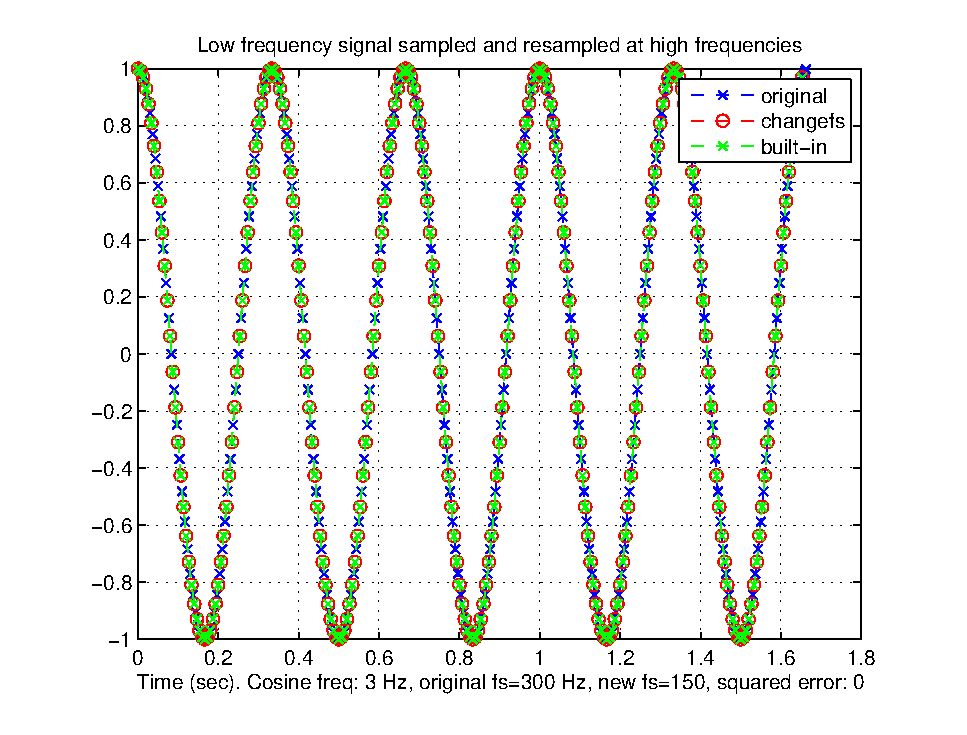
\includegraphics[width=0.4\paperwidth]{test11.eps}
\end{subfigure}
%~ \hfill
\begin{subfigure}[h]{0.49\textwidth}\centering
  \centering
  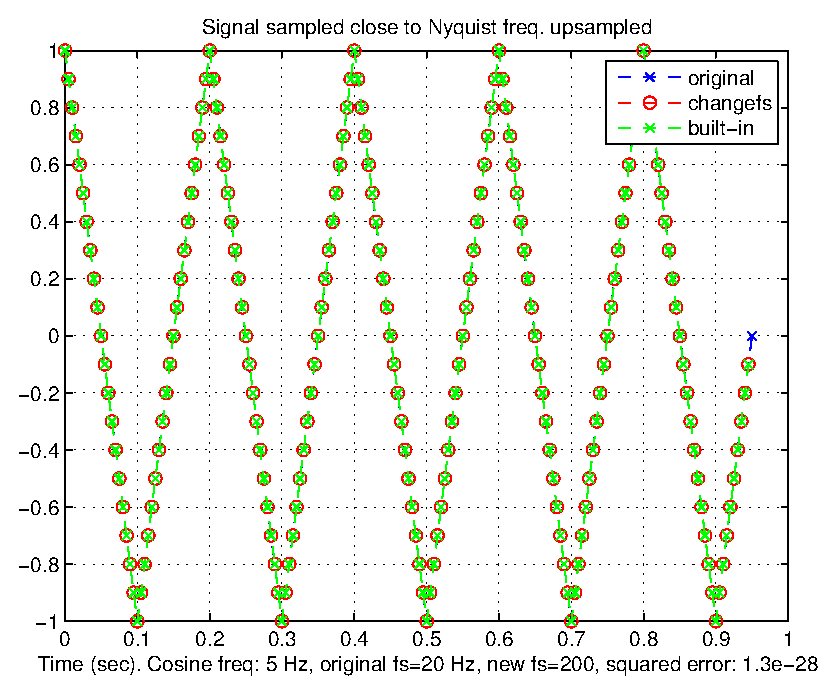
\includegraphics[width=0.4\paperwidth]{test12.eps}
  \end{subfigure}
  %~ \hfill
\begin{subfigure}[h]{0.49\textwidth}
  \centering
  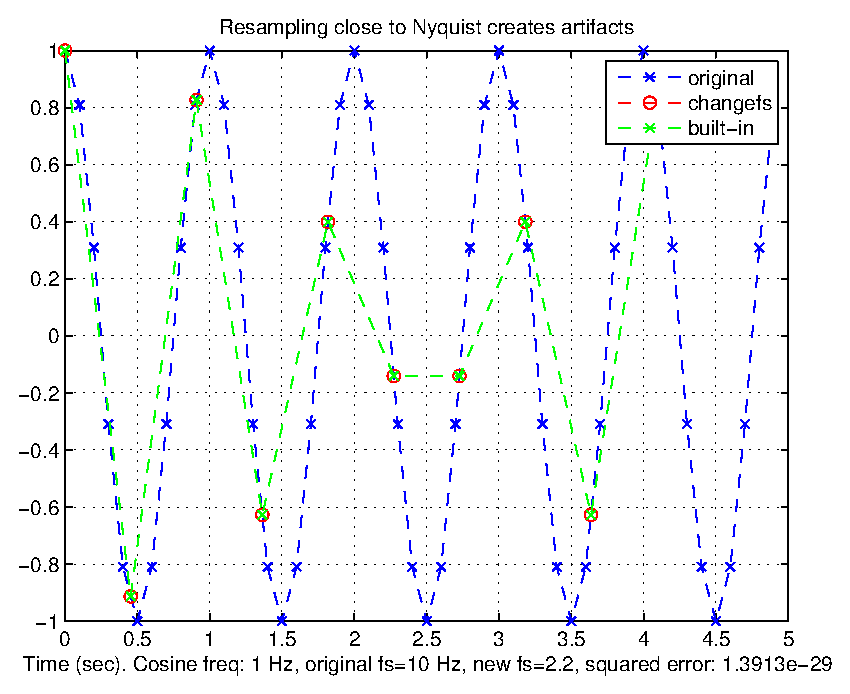
\includegraphics[width=0.4\paperwidth]{test13.eps}
\end{subfigure}
%~ \hfill
\begin{subfigure}[h]{0.49\textwidth}\centering
  \centering
  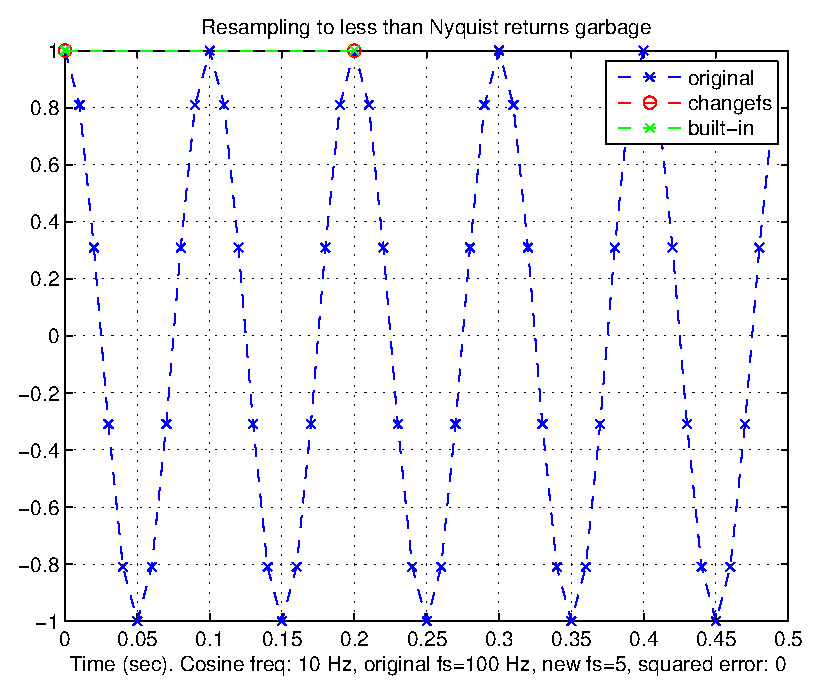
\includegraphics[width=0.4\paperwidth]{test14.eps}
  \end{subfigure}
  %~ \hfill
\end{figure}

\par Παρατηρούμε πως τα σημεία των καμπυλών built-in και changefs ταυτίζονται, 
άρα η υλοποίησή μας είναι σωστή.

\section{Σύστημα Γραμμικής Πρόβλεψης}

\section{Σύστημα Κβαντιστή \& Αποκβαντιστή}

\section{Κωδικοποίηση \& Αποκωδικοποίηση A-DPCM}

\section{Κωδικοποίηση \& Αποκωδικοποίηση Huffman}



\noindent
\begin{minipage}{\linewidth}
\par Το επόμενο βήμα για την υλοποίηση του συστήματος Κωδικοποιητή και Αποκωδικοποιητή που θέλουμε να
αναπτύξουμε είναι η κωδικοποίηση των συμβόλων που αποτελούν το σήμα μας και για αυτό το σκοπό
στρεφόμαστε στην χρήση του κώδικα Huffman.

  \par Ο αλγόριθμος του Huffman βασίζεται στις πιθανότητες εμφάνισης των συμβόλων που μας ενδιαφέρουν
  προκειμένου να εξάγει τον κώδικα που θα χρησιμοποιήσουμε για συμπίεση. Συγκεκριμένα, όσο πιο πιθανό
  είναι ένα σύμβολο, τόσο μικρότερη είναι η συμβολοσειρά που το αναπαριστά. Πρακτικά, μπορεί να
  αναπαρασταθεί από ένα δυαδικό δέντρο, όπου τα φύλλα αντιστοιχούν στα σύμβολα. Για την κατασκευή του
  δέντρου, ξεκινάμε από δύο στοιχεία που έχουν τη μικρότερη πιθανότητα, τα οποία κι ενώνουμε για να
  σχηματίσουμε έναν κόμβο του δέντρο, ο οποίος με την σειρά του θεωρείται ως ένα νέο σύμβολο, με
  πιθανότητα ίση με το άθροισμα των πιθανοτήτων των παιδιών. Στην συνέχεια, επιλέγουμε τα στοιχεία που
  έχουν τις δύο μικρότερες πιθανότητες κι επαναλαμβάνουν την παραπάνω διαδικασία. Ο αλγόριθμος
  τερματίζει όταν όλοι οι κόμβοι έχουν ενωθεί.
  \begin{framed}
    \begin{figure}[H]
      \label{fig:huffman}
      \centering
      \begin{subfigure}{1.0\textwidth}
        \centering
        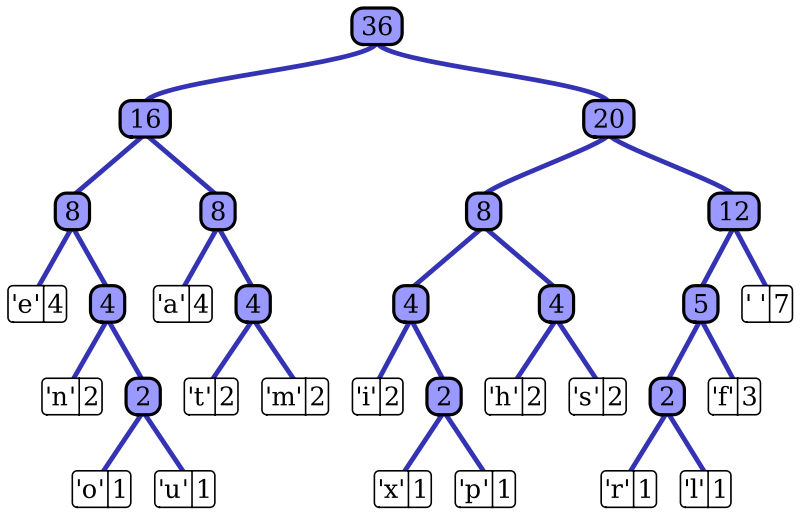
\includegraphics[width=0.8\textwidth]{huffman}
        \caption{\protect{Πηγή: \href{https://en.wikipedia.org/wiki/Huffman\_coding}{Huffman Wikipedia Article}}}
      \end{subfigure}
      \caption{Παράδειγμα Δέντρου Huffman}
    \end{figure}
  \end{framed}
\end{minipage}

\par Η συνάρτηση που κατασκευάζει το παραπάνω δέντρο και κατά συνέπεια και το λεξικό/σύνολο λέξεων
που μας δίνει τον κώδικα Huffman είναι η:
\begin{lstlisting}[style=myMatlab]
  function [s] = huffLUT(p, debug)
\end{lstlisting}
\noindent η οποία αρχικά δημιουργεί μία ουρά προτεραιότητας με κόμβους, όπου κάθε κόμβος είναι ένα
φύλλο που περιέχει ένα από τα αρχικά σύμβολα. Έπειτα, και για όσο υπάρχουν στοιχεία στην ουρά,
εξάγουμε τα δύο στοιχεία με τις χαμηλότερες πιθανότητες, τα ενώνουμε δημιουργώντας έναν νέο κόμβο,
όπως περιγράψαμε παραπάνω και τον οποίο εισάγουμε στην ουρά, αναθέτοντας του και το αντίστοιχο
ψηφίο. Για να εξάγουμε τον κώδικα που αντιστοιχεί σε κάθε σύμβολο, απλά ξεκινάμε από το αντίστοιχο
φύλλο κι ανεβαίνουμε μέχρι την ρίζα του δέντρου, κρατώντας τα ψηφία των κόμβων από τους οποίους
περνάμε.

\par Η συνάρτηση:
\begin{lstlisting}[style=myMatlab]
  function [b] = huff(q, s)
\end{lstlisting}
\noindent κωδικοποιεί την συμβολοσειρά που μας δίνεται με βάση το λεξιλόγιο που δημιούργησε η
\emphcolor{huffLut} αντιστοιχώντας κάθε σύμβολο στον κώδικα του.

\par Τέλος, η συνάρτηση:
\begin{lstlisting}[style=myMatlab]
  function [q, n] = ihuff(b, s, debug)
\end{lstlisting}
\noindent εκτελεί τον αντίστροφο μετασχηματισμό Huffman δοθέντος του λεξιλογίου και μίας σειράς
ψηφίων. Για να το πετύχει αυτό δημιουργεί το δέντρο Huffman από τις κωδικολέξεις, εκτελώντας
έναν βρόγχο for για κάθε μία από αυτές. Αρχικά, δημιουργούμε έναν κενό κόμβο, ο οποίος και αποτελεί
την ρίζα του δέντρου μας. Στην συνέχεια, για κάθε κωδικολέξη, εξετάζουμε ένας προς ένα τα ψηφία της
και δημιουργούμε έναν νέο κόμβο για το καθένα εφόσον δεν υπάρχει, στα δεξιά τρέχοντος κόμβου αν
είναι το 0, διαφορετικά στα αριστερά, προχωρώντας μέχρι να εξαντλήσουμε τα bits της. Όταν εξετάσουμε
το σύνολο του λεξιλογίου θα έχουμε κατασκευάσει ξανά το δέντρο Huffman.
\par Προκειμένου να αποκωδικοποιήσουμε το bitstream που μας δίνεται, εισάγουμε τα bits του στο
δέντρο. Μόλις βρεθούμε σε κάποιο φύλλο προσθέτουμε στο τέλος της αποκωδικοποιημένης πρότασης μας το
αντίστοιχο σύμβολο. Αν στο τέλος της σειράς των bits δεν βρισκόμαστε σε φύλλο τότε επιστρέφουμε και
τον αριθμό των μηδενικών και άσσων που περίσσεψαν.


\end{document}
